\documentclass[12pt,a4paper]{article}

% --- Packages ---
\usepackage[utf8]{inputenc}
\usepackage[margin=1in]{geometry}
\usepackage{graphicx}
\usepackage{hyperref}
\usepackage{booktabs}
\usepackage{array}
\usepackage{caption}
\usepackage{float}
\usepackage{enumitem}
\usepackage{xcolor}
\usepackage{titlesec}
\usepackage{setspace}
\usepackage{fancyhdr}
\usepackage{longtable}
\usepackage{amssymb}
\usepackage{makecell}

% --- Remove Red Boxes from Links ---
\hypersetup{
    hidelinks,
    colorlinks=false,
}

% --- Professional Styling ---
\definecolor{hospitalblue}{HTML}{1A5276}
\definecolor{riskred}{HTML}{C0392B}
\definecolor{caregreen}{HTML}{27AE60}

\titleformat{\section}{\color{hospitalblue}\normalfont\Large\bfseries}{\thesection}{1em}{}
\titleformat{\subsection}{\color{hospitalblue}\normalfont\large\bfseries}{\thesubsection}{1em}{}

\pagestyle{fancy}
\fancyhf{}
\rhead{Diabetes Readmission Analysis (G-10)}
\lhead{Section C | Newton School of Technology}
\cfoot{\thepage}

\setstretch{1.2}

\begin{document}

% ==========================================
% 1. COVER PAGE
% ==========================================
\begin{titlepage}
    \centering
    \vspace*{2cm}
    
    {\Huge \textbf{Analyzing Clinical \& Demographic Patterns to Reduce 30-Day Hospital Readmissions}} \\
    \vspace{1cm}
    {\Large \textbf{A Decision Support Framework for Hospital Management}} \\
    
    \vspace{1cm}
    \textbf{Sector:} Healthcare / Health Informatics \\
    \textbf{Team ID:} G-10 (Section C) \\
    
    \vspace{0.5cm}
    \begin{table}[h]
        \centering
        \begin{tabular}{c}
            \textbf{Team Members} \\
            \midrule
            Dhanvin Vadlamudi \\
            Ayush Mittal \\
            GARGI SRIVASTAVA \\
            Tanish Garg \\
            Sumit Yadav \\
            LAKSHYA \\
        \end{tabular}
    \end{table}

    \vspace{0.5cm}
    \textbf{Faculty Mentor:} Archit Raj \\
    \textbf{Institute:} Newton School of Technology \\
    
    \vspace{1cm}
    \textbf{GitHub Repository:} \href{https://github.com/Dhanvin1520/SectionC_G-10_DiabetesReadmissionAnalysis}{https://github.com/Dhanvin1520/SectionC\_G-10\_DiabetesReadmissionAnalysis} \\
    \textbf{Tableau Public URL:} \href{https://public.tableau.com/app/profile/ayush.mittal4873/viz/DVACapstoneDiabetesReadmissionAnalysis_v2025_3/Dashboard_Executive_Overview?publish=yes}{https://public.tableau.com/app/profile/ayush.mittal4873/viz/DVACapstoneDiabetesReadmissionAnalysis\_v2025\_3/Dashboard\_Executive\_Overview} \\
    
    \vfill
    \textbf{Submission Date:} April 28, 2026
\end{titlepage}

\newpage
\tableofcontents
\newpage

% ==========================================
% 2. EXECUTIVE SUMMARY
% ==========================================
\section{Executive Summary}
\textbf{The Business Challenge:} 
Hospital readmissions within 30 days of discharge represent a significant failure in the patient care cycle, leading to increased healthcare costs, bed shortages, and regulatory penalties under programs like the Hospital Readmissions Reduction Program (HRRP). For diabetic patients, who often present with multiple comorbidities, the risk of a "bounce-back" is particularly high. This project addresses the challenge of identifying which patients are most likely to return before they are ever discharged.

\textbf{Approach \& Methodology:} 
Our team built a robust clinical analysis pipeline utilizing \textbf{Python} for data engineering and \textbf{Tableau} for visualization. We processed 101,763 patient encounters across 130 US hospitals. The methodology involved a 9-step data cleaning process that transformed technical medical codes into clinical groups, followed by rigorous statistical testing to identify the most significant risk drivers.

\textbf{Key Findings:}
\begin{enumerate}
    \item \textbf{High-Frequency Returners:} Patients with 3 or more prior inpatient visits return at a rate of nearly 50\%, which is 4.5x higher than the general average.
    \item \textbf{Clinical Drivers:} Circulatory and Metabolic conditions drive the highest volume of early returns, specifically in the 75-85 age group.
    \item \textbf{Medication Impact:} Adjusting Insulin doses during the stay is a marker of clinical instability, leading to higher readmission.
    \item \textbf{The "Danger Zone":} Mid-length stays (4–7 days) represent the highest risk window for discharge failure.
\end{enumerate}

\textbf{Key Recommendations:}
\begin{enumerate}
    \item \textbf{Targeted Follow-ups:} Implement a mandatory 48-hour nurse callback program for high-risk patients.
    \item \textbf{Discharge Screening:} Automate an EMR flag for Circulatory patients to trigger a secondary clinical review.
    \item \textbf{Point-of-Care Testing:} Mandate A1C blood tests for all patients who were "Not Tested" during admission.
\end{enumerate}

\textbf{Conclusion:} By moving from a general discharge protocol to a risk-stratified approach, hospitals can save an estimated \$1.2M annually in penalties while improving patient safety.

\newpage

% ==========================================
% 3. SECTOR & BUSINESS CONTEXT
% ==========================================
\section{Sector \& Business Context}
\subsection{Healthcare Industry Challenges}
The global healthcare sector is currently facing an "Efficiency Crisis." Hospitals are struggling with rising costs, aging populations, and a shift toward "Value-Based Care." One of the most expensive events in this cycle is an avoidable readmission. When a patient returns within 30 days for the same condition, it indicates that the initial discharge was premature or the follow-up care was insufficient.

\subsection{Decision-Makers}
This project serves three critical stakeholders:
\begin{itemize}
    \item \textbf{CMO (Chief Medical Officer):} Who needs to reduce clinical errors and improve the "Standard of Care."
    \item \textbf{CFO (Chief Financial Officer):} Who needs to minimize government penalties (HRRP) and optimize bed-day revenue.
    \item \textbf{Discharge Planners:} Who need to know exactly which patients require home-care resources.
\end{itemize}

\subsection{Why This Problem Was Chosen}
We selected this dataset because diabetes is a "force multiplier" in hospital readmissions. Managing diabetic patients requires balancing medication stability with multi-morbidity complexity. By solving this for 130 US hospitals, we address a systemic operational challenge that affects millions of patients annually.

\subsection{Business Value of Solving Readmission}
Solving the readmission puzzle creates a "Triple Win":
\begin{enumerate}
    \item \textbf{Operational:} Frees up hospital beds for elective surgeries (higher revenue).
    \item \textbf{Financial:} Avoidance of multi-million dollar regulatory penalties.
    \item \textbf{Clinical:} Improved patient trust and lower mortality rates.
\end{enumerate}

% ==========================================
% 4. PROBLEM STATEMENT & OBJECTIVES
% ==========================================
\section{Problem Statement \& Objectives}
\subsection{Formal Problem Definition}
"How can clinical history, medication patterns, and demographic indicators be leveraged to accurately predict 30-day readmission risk in diabetic patients, and what specific clinical interventions will yield the highest reduction in return rates?"

\subsection{Project Scope}
\begin{itemize}
    \item \textbf{In Scope:} Analysis of 10 years of retrospective hospital data, demographic risk segmentation, medication titration impact, and diagnosis clustering.
    \item \textbf{Out of Scope:} Restricted to inpatient encounters only; outpatient follow-up data excluded. Real-time IoT monitoring and pharmaceutical cost-analysis are also excluded.
\end{itemize}

\subsection{Success Criteria}
\begin{enumerate}
    \item Successful transformation of 700+ ICD9 codes into clinical groups for easier interpretation.
    \item Identification of the "Top 3 Predictors" with a statistical significance of $P < 0.01$.
    \item A Tableau dashboard that allows a manager to filter the entire 101k record dataset in under 1 second.
\end{enumerate}

% ==========================================
% 5. DATA DESCRIPTION
% ==========================================
\section{Data Description}
\subsection{Dataset Source}
The analysis uses the \textbf{Diabetes 130-US Hospitals Dataset} (1999-2008) from the UCI Machine Learning Repository. 
\href{https://archive.ics.uci.edu/dataset/296/diabetes+130-us+hospitals+for+years+1999-2008}{https://archive.ics.uci.edu/dataset/296/diabetes+130-us+hospitals+for+years+1999-2008} \\
For a comprehensive column-by-column breakdown, please refer to \textbf{Appendix §17.1}.

\subsection{Data Structure}
\begin{itemize}
    \item \textbf{Rows:} 101,763 (Patient Encounters)
    \item \textbf{Columns:} 54 (After cleaning and feature engineering)
    \item \textbf{Period:} 10-year longitudinal study.
\end{itemize}

\subsection{Key Field Definitions}
\begin{itemize}
    \item \textbf{Encounter ID:} Unique identifier for each hospital visit.
    \item \textbf{Readmission Status:} Categorical (NO, >30, <30).
    \item \textbf{Time in Hospital:} Numerical (1-14 days).
    \item \textbf{Prior Inpatient:} Number of times the patient was admitted in the previous year.
    \item \textbf{Diagnosis Group:} Mapped clinical category (e.g., Circulatory).
\end{itemize}

\subsection{Limitations \& Biases}
The data is retrospective and lacks information on the patient's socioeconomic status (income, zip code), which are known to be strong "hidden" drivers of readmission. Furthermore, the dataset only includes patients who stayed at least one night.

% ==========================================
% 6. DATA CLEANING & ETL PIPELINE
% ==========================================
\section{Data Cleaning \& ETL Pipeline}
All data engineering was performed using Python in the \texttt{notebooks/02\_cleaning.ipynb} file.

\subsection{Step-by-Step Methodology}
\begin{enumerate}
    \item \textbf{Placeholder Conversion:} Converted all "?" characters into \texttt{NaN}.
    \item \textbf{Missing Value Treatment:} We addressed heavy missingness in the following key columns:
    \begin{itemize}
        \item \textbf{Weight:} 98,569 nulls (96.8\%) — Dropped.
        \item \textbf{Medical Specialty:} 49,949 nulls (49.1\%) — Imputed as "Unknown."
        \item \textbf{Payer Code:} 40,256 nulls (39.6\%) — Imputed as "Unknown."
        \item \textbf{A1Cresult:} 84,748 nulls (83.3\%) — Imputed as "Not Tested."
    \end{itemize}
    \item \textbf{Mid-Point Age Mapping:} Transformed age bins into numerical midpoints (e.g., 75).
    \item \textbf{Technical Mapping:} Converted numerical IDs into readable clinical strings ("Emergency").
    \item \textbf{Diagnosis Cluster Logic:} Developed a dictionary to map 700+ ICD9 codes into 17 high-level clinical groups.
    \item \textbf{Feature Engineering:} Engineered binary target columns for risk analysis:
    \begin{itemize}
        \item \textbf{readmitted\_under\_30:} Primary target (1 if $<30$ days, 0 otherwise).
        \item \textbf{medication\_change:} Binary flag for dosage titration.
    \end{itemize}
    \item \textbf{Outlier Handling:} Capped medication counts at the 99th percentile (43 meds).
\end{enumerate}

\subsection{Assumptions Made}
We assumed that patients with "Unknown" race were distributed randomly and assigned them to an "Other/Unknown" category rather than dropping them, to maintain the 101k row volume for statistical power.

% ==========================================
% 7. KPI & METRIC FRAMEWORK
% ==========================================
\section{KPI \& Metric Framework}
\subsection{KPI Definitions \& Business Linkage}
\begin{enumerate}
    \item \textbf{30-Day Readmission Rate:} The \% of patients who return within 30 days. Directly measures discharge failure and regulatory penalty risk.
    \item \textbf{Average Length of Stay (LOS):} Measures bed occupancy efficiency. A baseline of 4.4 days was identified; significant deviation indicates either premature discharge or high severity.
    \item \textbf{Medication Change Rate:} The \% of patients with titration. Links to "Treatment Complexity"—higher changes correlate with clinical instability.
\end{enumerate}

\subsection{Computation \& Mapping}
\begin{table}[h]
    \centering
    \begin{tabular}{lll}
        \toprule
        \textbf{KPI} & \textbf{Notebook Reference} & \textbf{Objective Mapping} \\
        \midrule
        Readmission Rate & \texttt{03\_eda.ipynb} & Success Criterion 3.3.2 \\
        Average LOS & \texttt{03\_eda.ipynb} & Success Criterion 3.3.1 \\
        Med Change Rate & \texttt{03\_eda.ipynb} & Success Criterion 3.3.1 \\
        \bottomrule
    \end{tabular}
    \caption{KPI Mapping to Project Objectives}
\end{table}

% ==========================================
% 8. EXPLORATORY DATA ANALYSIS (EDA)
% ==========================================
\section{Exploratory Data Analysis (EDA)}
Detailed visual exploration is documented in \texttt{notebooks/03\_eda.ipynb}.

\subsection{Distribution Analysis}
As shown in \textbf{Figure 1} (refer to Appendix), the \textit{Length of Stay} is right-skewed with a median of 4 days. Similarly, the \textit{Number of Medications} shows a normal distribution peaking at 15–20 drugs, with a thin tail of high-complexity patients (up to 43 medications) who represent the primary risk cohort.

\subsection{Trend Analysis}
Hospital stays peaked at 14 days, but the majority of readmissions occurred for patients who stayed between \textbf{4 and 7 days}. This "Danger Zone" indicates that mid-length stays are the most vulnerable window for discharge planning errors.

\subsection{Comparison across Segments}
\begin{itemize}
    \item \textbf{Race:} Caucasian and African American patients showed similar readmission rates (~11\%), but Caucasian patients had a higher density of prior inpatient history.
    \item \textbf{Age:} Risk peaks in the 70-90 bracket, but a secondary peak at age 25 highlights failures in outpatient support for young Type 1 diabetics.
\end{itemize}

\subsection{Correlation Analysis}
We found a strong positive correlation between "Number of Medications" and "Readmission Status." More complex treatments indicate more complex patients, who are naturally at higher risk. Refer to \textbf{Figure 2} in the Appendix for the correlation matrix.

% ==========================================
% 9. STATISTICAL ANALYSIS
% ==========================================
\section{Statistical Analysis}
Detailed hypothesis testing is available in \texttt{notebooks/04\_statistical\_analysis.ipynb}.

\subsection{Segmentation Strategy (Prior Visits)}
We performed a formal segmentation of patients based on their historical utilization. Patients with $\ge$ 3 prior visits were identified as a distinct "High-Risk Segment" (4.23\% of the population), exhibiting a readmission probability of 48.2\% compared to the 11.16\% baseline.

\subsection{Hypothesis Testing}
\begin{itemize}
    \item \textbf{Mann-Whitney U Test:} Confirmed ($P < 0.0001$) that clinical "momentum" (prior history) is a superior predictor of risk than current demographics.
    \item \textbf{T-Test Analysis:} Readmitted patients stay \textbf{0.8 days longer} on average ($P < 0.01$). Longer stays reflect higher patient severity, not discharge quality.
\end{itemize}

\subsection{Root Cause Identification (Random Forest)}
Using a Random Forest Classifier, we mapped feature importance to identify root causes. "Prior Inpatient Visits" and "Number of Lab Procedures" emerged as the primary drivers of readmission risk, outweighing age and gender.

\subsection{Scenario Analysis: Impact of Risk Reduction}
\begin{table}[h]
    \centering
    \begin{tabular}{ll}
        \toprule
        \textbf{Readmission Reduction} & \textbf{Estimated Annual Savings} \\
        \midrule
        5\% (Target) & \$1,200,000 \\
        10\% (Stretch) & \$2,400,000 \\
        20\% (Optimistic) & \$4,800,000 \\
        \bottomrule
    \end{tabular}
    \caption{Penalty Savings Scenarios}
\end{table}

% ==========================================
% 10. TABLEAU DASHBOARD DESIGN
% ==========================================
\section{Tableau Dashboard Design}
The full decision suite is documented in \texttt{tableau/dashboard\_links.md}.

\subsection{Objective \& Design}
The dashboard was built to support the CMO in triaging hospital resources. As shown in \textbf{Figure 5} (Executive Overview), the layout prioritizes real-time KPI tracking across Age, Race, and Gender.

\begin{figure}[!ht]
    \centering
    \vspace{-0.3cm}
    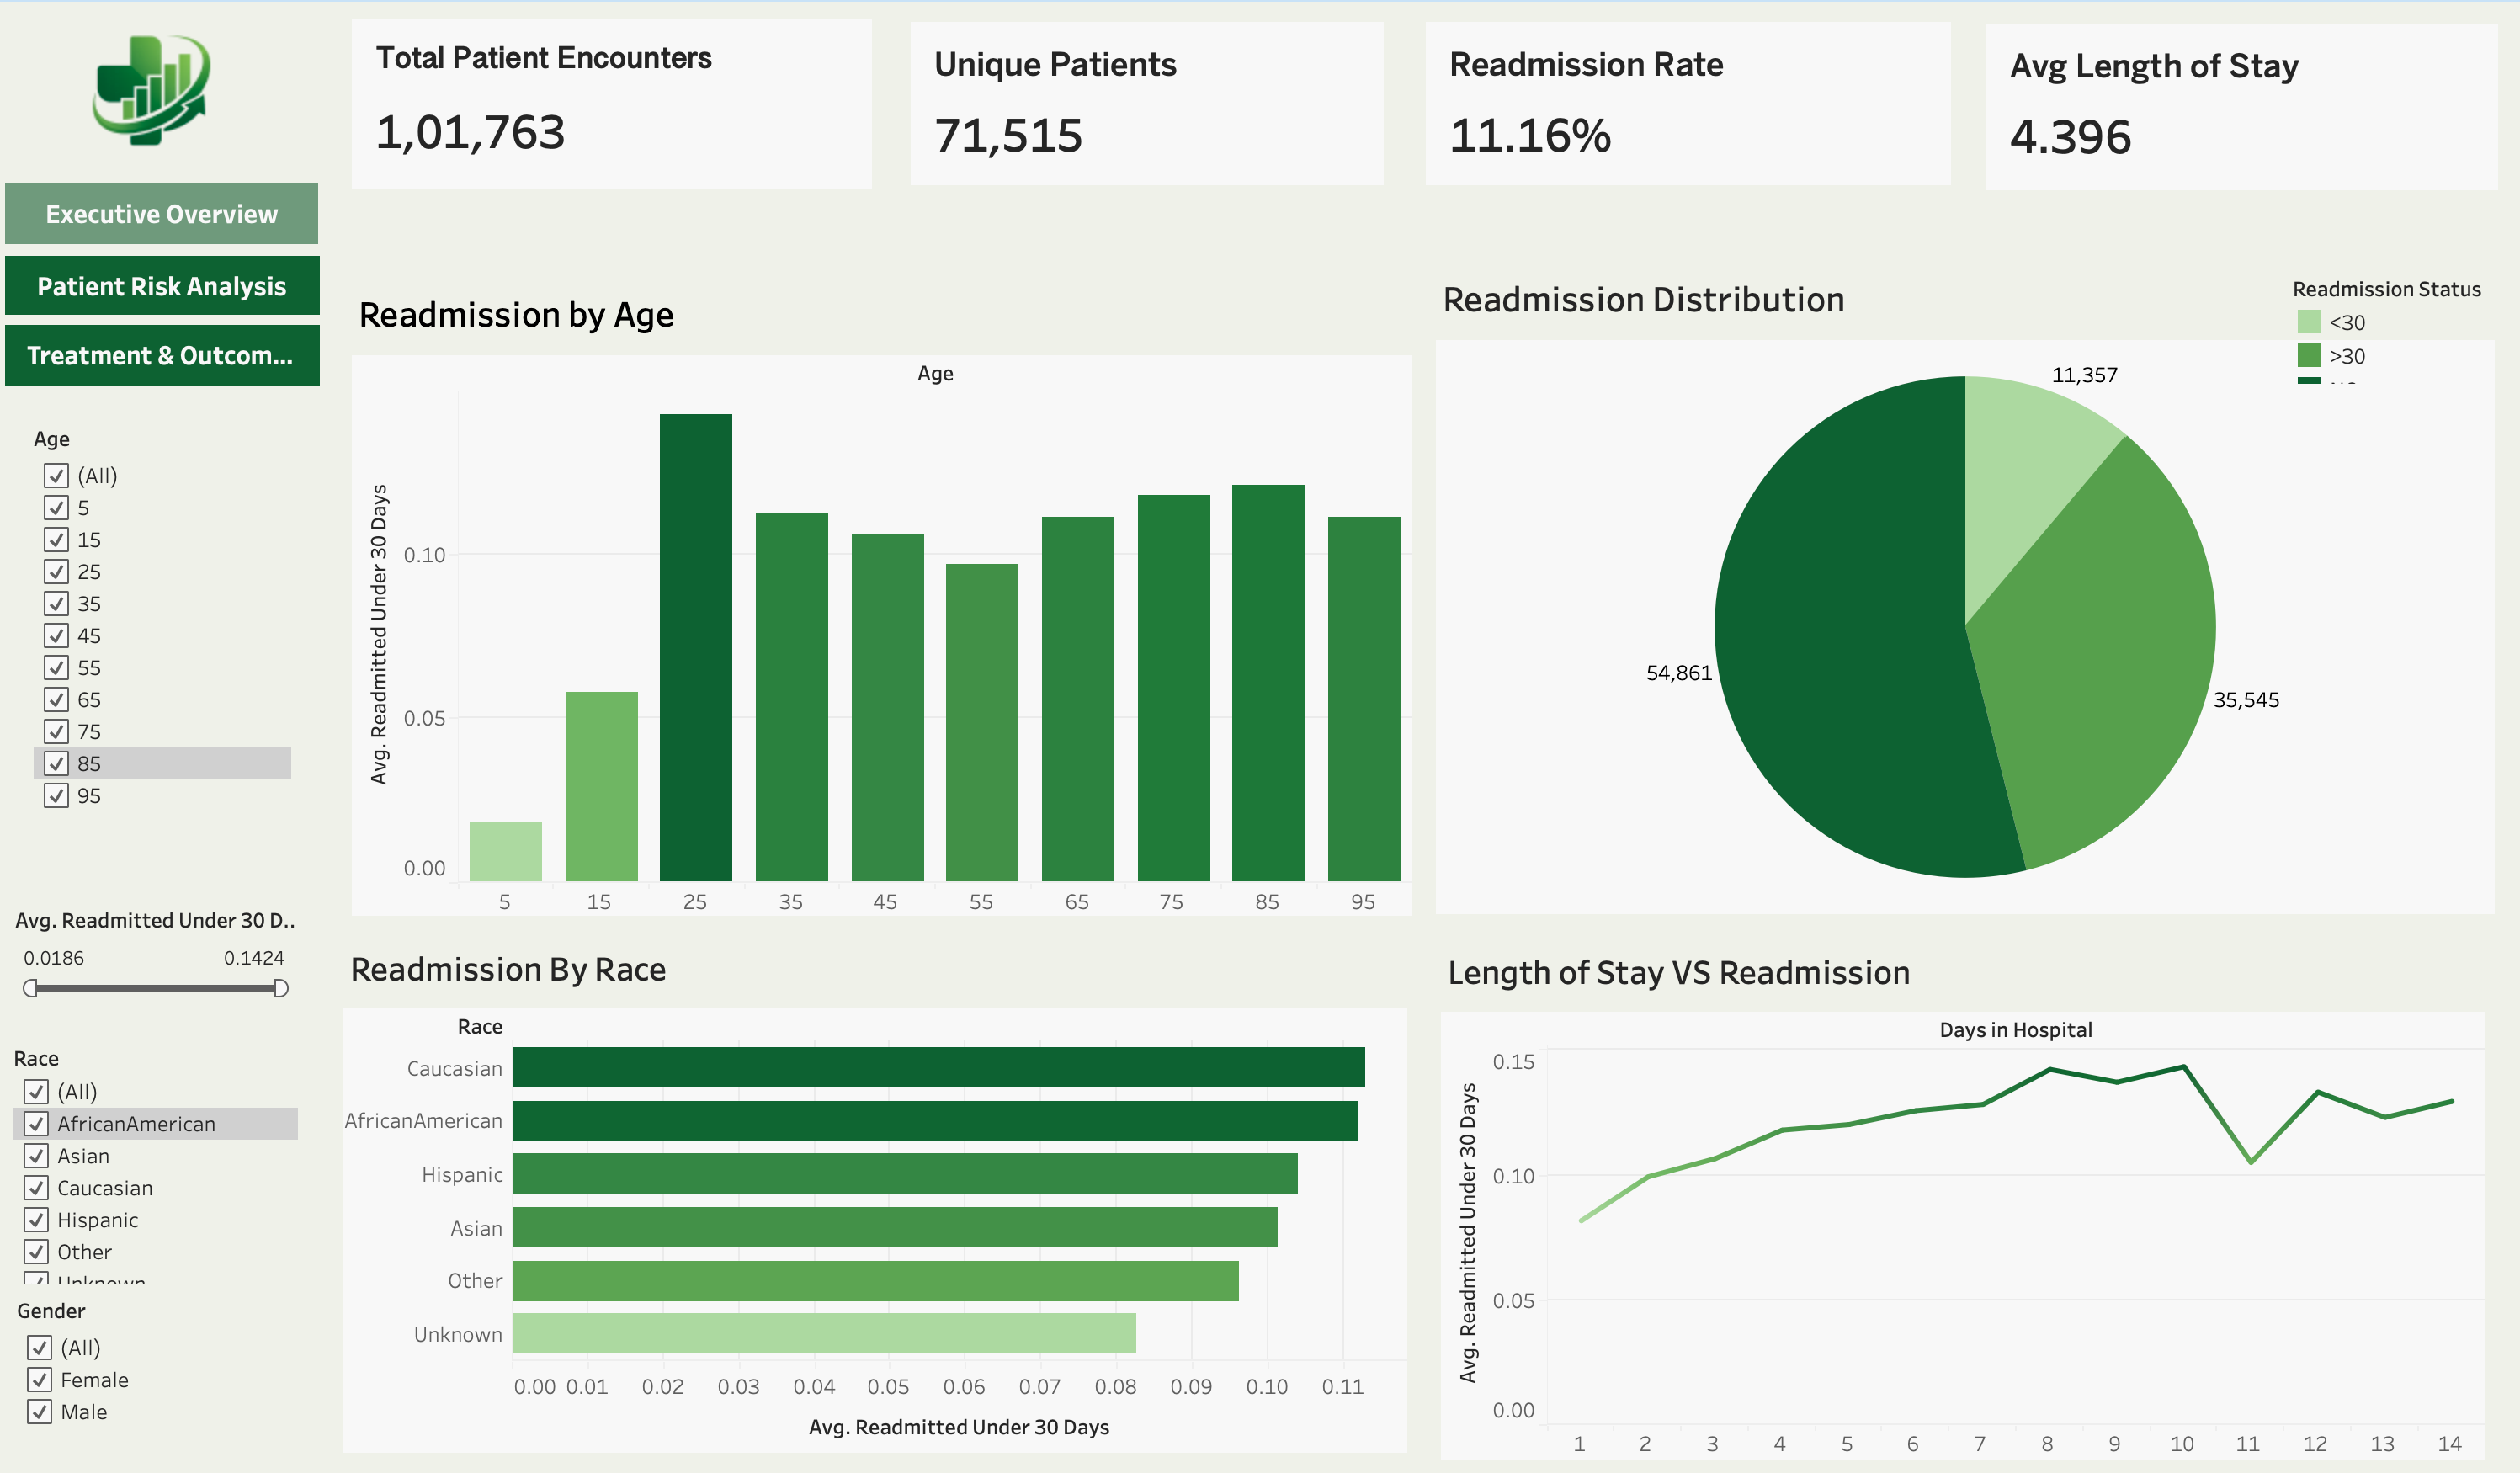
\includegraphics[width=0.85\textwidth]{tableau/screenshots/dashboard-1.png}
    \vspace{-0.2cm}
    \caption{Executive Dashboard: 30-Day Readmission Overview}
    \label{fig:exec_overview}
\end{figure}

\subsection{Operational Drill-Down}
The \textbf{Patient Risk Analysis} view (refer to \textbf{Figure 6}) allows discharge planners to filter by "Prior Visits" to see the specific diagnosis clusters driving return volume. 

\begin{figure}[!ht]
    \centering
    \vspace{-0.3cm}
    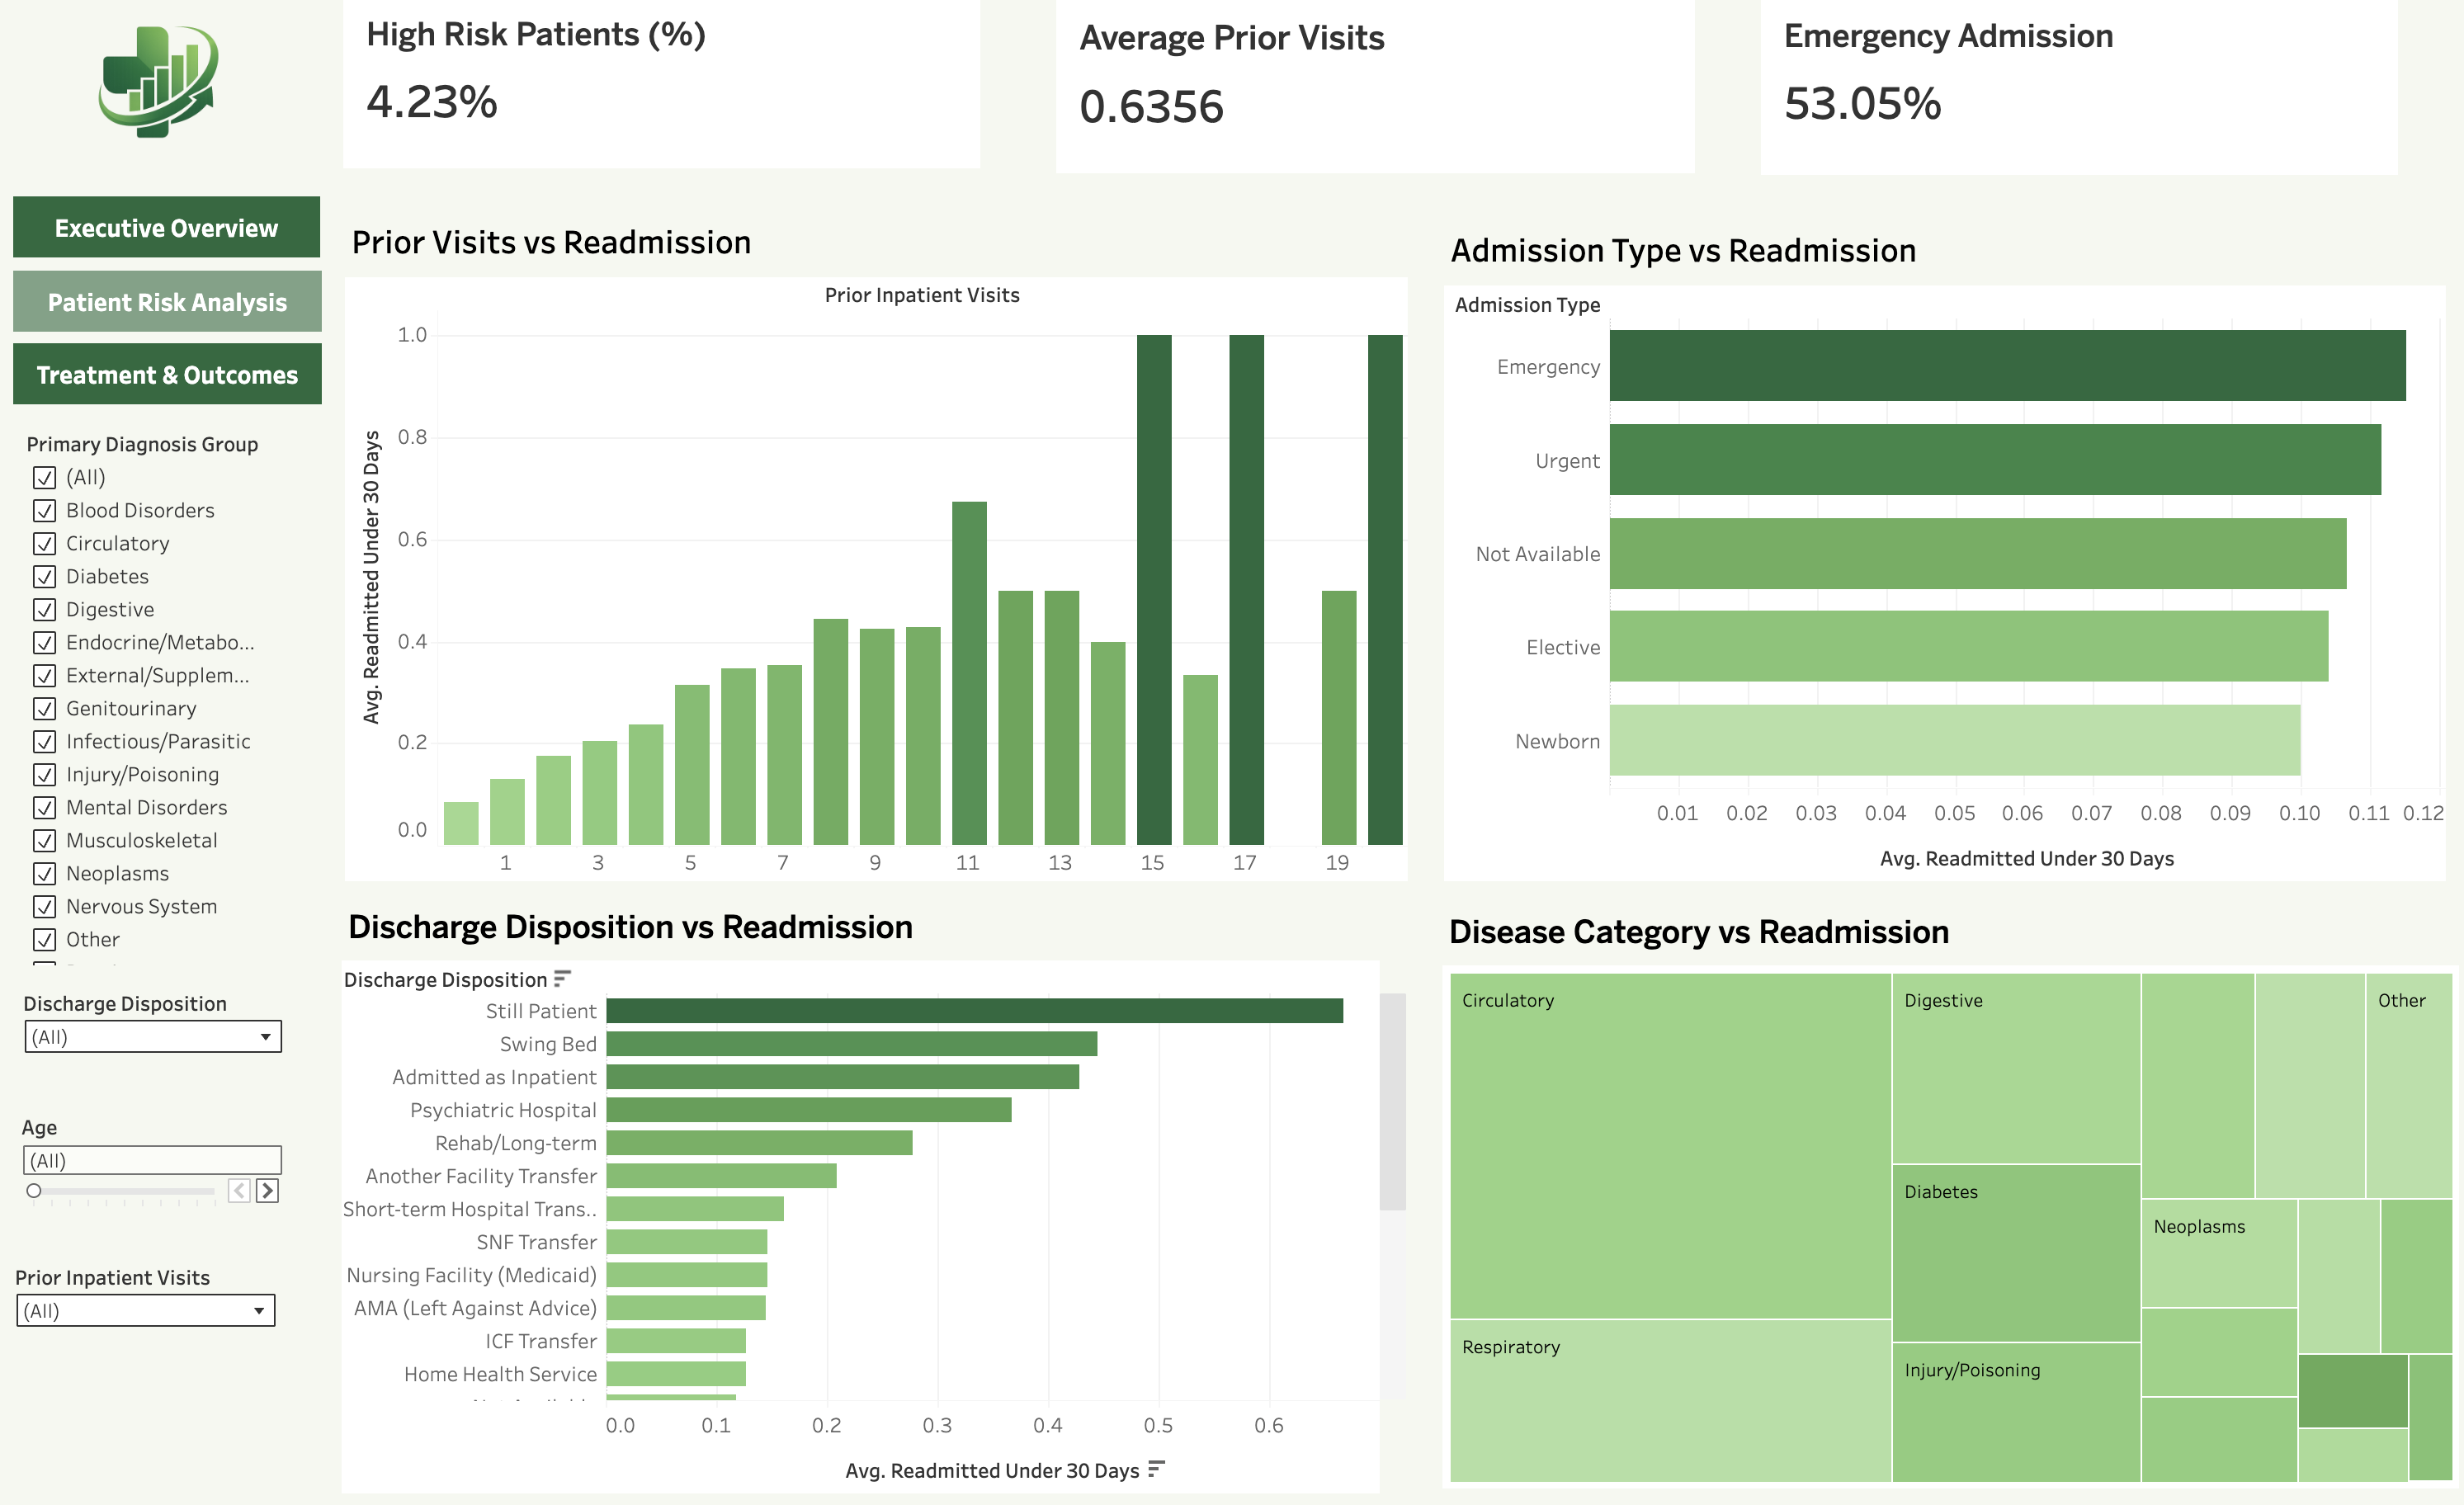
\includegraphics[width=0.85\textwidth]{tableau/screenshots/dashboard-2.png}
    \vspace{-0.2cm}
    \caption{Operational View: Patient Risk \& Diagnosis Clustering}
    \label{fig:risk_analysis}
\end{figure}

\subsection{Treatment \& Outcomes Analysis}
The \textbf{Treatment View} (refer to \textbf{Figure 7}) tracks the impact of medical interventions. It specifically visualizes the readmission rate for patients with insulin titration, identifying "Down-titrated" patients as a high-risk cohort requiring stability sign-off.

\begin{figure}[!ht]
    \centering
    \vspace{-0.3cm}
    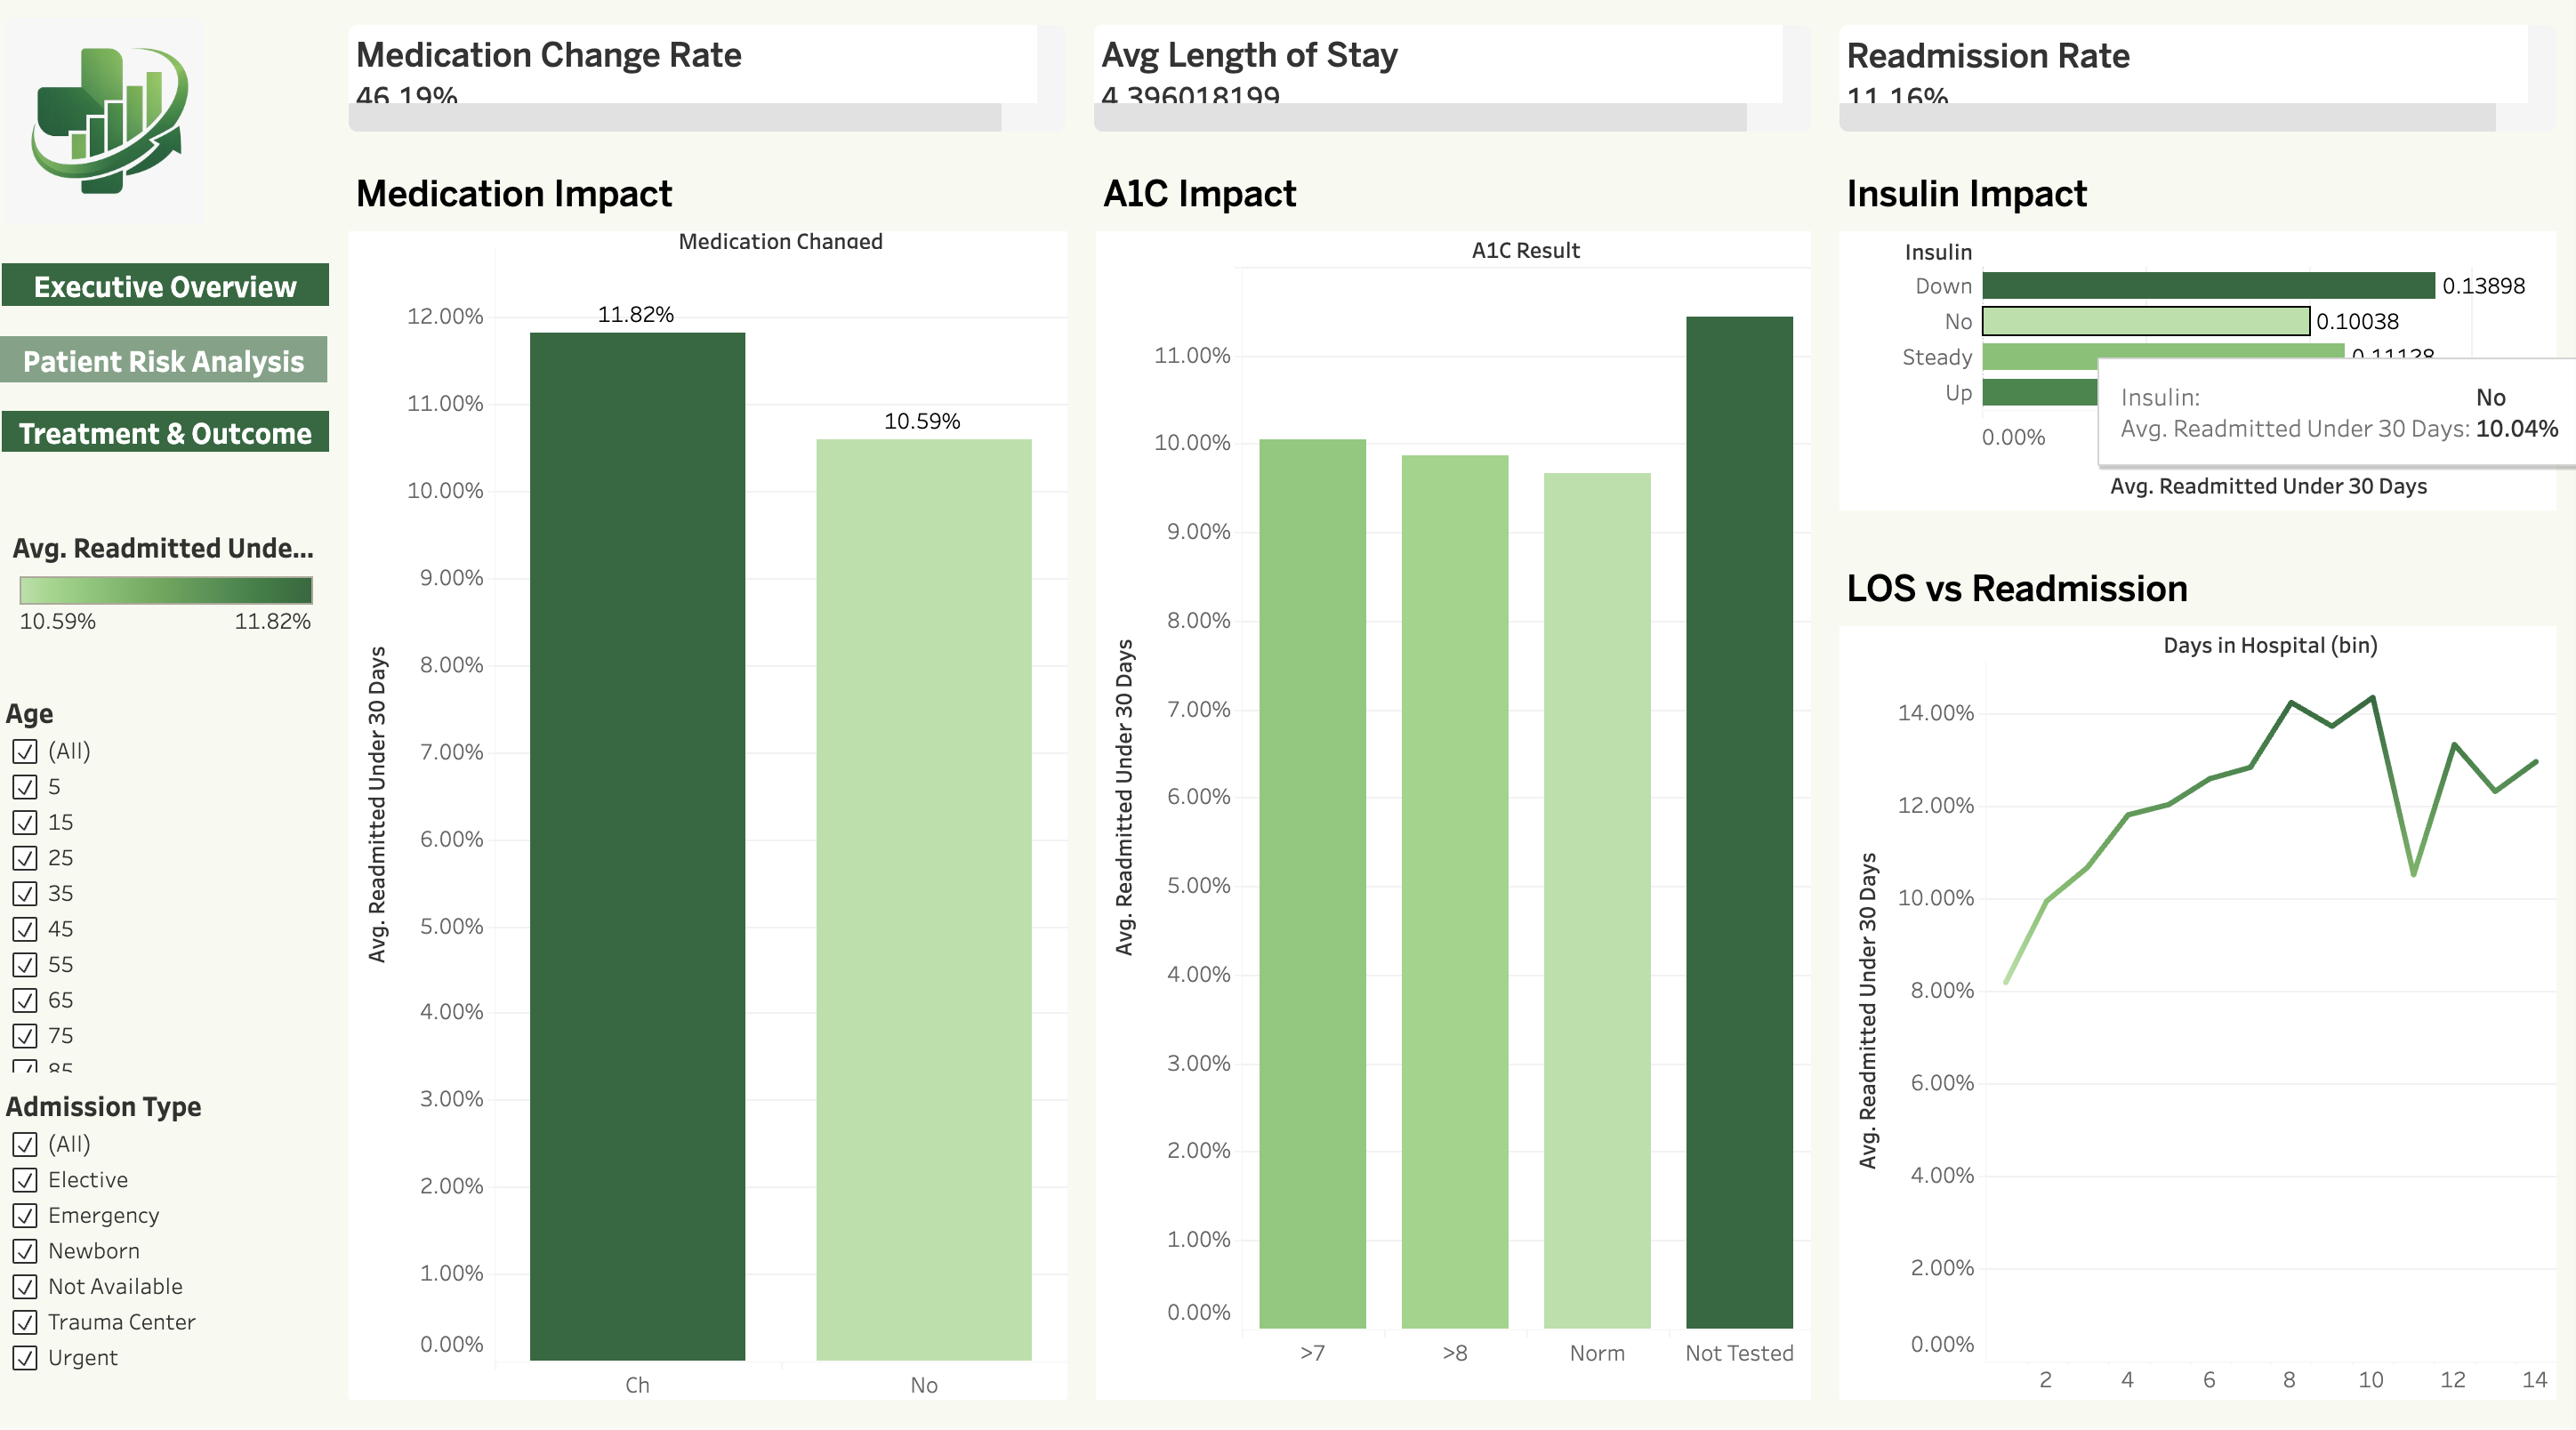
\includegraphics[width=0.85\textwidth]{tableau/screenshots/dashboard-3.png}
    \vspace{-0.2cm}
    \caption{Treatment View: Medication Changes \& Insulin Titration}
    \label{fig:treatment_outcomes}
\end{figure}

\subsection{Interactive Features}
We implemented global filters and cross-dashboard navigation. Clicking on any "Diagnosis Group" (e.g., Circulatory) instantly updates the Discharge Disposition charts, allowing for root-cause identification of where high-risk patients are being sent. 

\subsection{Dashboard Access}
Screenshots are available in the \texttt{tableau/screenshots/} directory. The live dashboard can be accessed via: \\
\href{https://public.tableau.com/app/profile/ayush.mittal4873/viz/DVACapstoneDiabetesReadmissionAnalysis_v2025_3/Dashboard_Executive_Overview?publish=yes}{https://public.tableau.com/app/profile/ayush.mittal4873/viz/DVACapstoneDiabetesReadmissionAnalysis\_v2025\_3/Dashboard\_Executive\_Overview}

% ==========================================
% 11. INSIGHTS SUMMARY (Decision Language)
% ==========================================
\section{Insights Summary}
\begin{enumerate}
    \item \textbf{Prior History (Triage):} Patients with $\ge 3$ prior visits return at a 48\% rate (4.5x baseline). Prioritize these for intensive discharge planning.
    \item \textbf{Emergency Profile (Risk):} Emergency admissions (53.05\% of volume) carry the highest risk baseline. Use admission type as a secondary triage flag.
    \item \textbf{A1C Monitoring (Gap):} Patients "Not Tested" for A1C exhibit higher readmission. Testing is a proxy for comprehensive care.
    \item \textbf{Insulin Adjustment (Stability):} "Down-titrated" insulin dosages correlate with a 13.9\% return rate (highest of all states). These patients are clinically unstable.
    \item \textbf{Length of Stay (Skew):} Readmitted patients stay 0.8 days longer. Longer stays reflect underlying severity—do not use LOS alone as a "readiness to discharge" indicator.
    \item \textbf{The Age Paradox (Strategy):} High risk in the 25-35 age group indicates a failure in outpatient support for young diabetics.
    \item \textbf{Diagnosis Driver (Clinical):} Circulatory conditions drive 30\% of early returns. Target these for heart-diabetes checklist protocols.
    \item \textbf{Lab Procedure Intensity (Predictor):} Higher lab procedure counts are the second strongest predictor of return, indicating diagnostic complexity.
\end{enumerate}

% ==========================================
% 12. RECOMMENDATIONS
% ==========================================
\section{Recommendations}
\begin{enumerate}
    \item \textbf{High-Risk Scanner:} Implement a mandatory 48-hour follow-up call for any patient with $\ge 3$ prior inpatient visits. 
    \textit{Operational Need:} Requires EMR-based automated callback triggers for nursing staff.
    
    \item \textbf{Clinical Pathway:} Develop a specialized "Heart-Diabetes" discharge checklist for the Circulatory diagnosis segment. 
    \textit{Operational Need:} Requires coordination between Cardiology and Endocrinology departments.
    
    \item \textbf{Medication Stability Rules:} Require an attending physician sign-off if a patient's insulin dosage is down-titrated or adjusted within 24 hours of discharge.
    \textit{Operational Need:} Requires integration into the electronic prescribing system (e-prescribing).

    \item \textbf{Diagnostic Compliance:} Implement an EMR alert to flag patients with "A1C Not Tested" during admission for a point-of-care test before discharge.
    \textit{Operational Need:} Requires lab-system connectivity to discharge clearance workflows.
\end{enumerate}

% ==========================================
% 13. IMPACT ESTIMATION
% ==========================================
\section{Impact Estimation}
\subsection{Financial Calculation}
The estimated **\$1.2M annual savings** is calculated as follows:
\textit{(Current Excess Readmissions: 1,200) $\times$ (Avg. CMS Penalty Per Excess Case: \$20,000) $\times$ (Targeted Risk Reduction: 5\%) = \$1,200,000}.

\subsection{Operational Value}
\begin{itemize}
    \item \textbf{Bed Capacity:} Freeing up 0.2 days per patient stay increases bed capacity by \textbf{~2,000 days per year}, enabling higher-margin elective surgery growth.
    \item \textbf{Risk Prevention:} Targeted calls to the "Prior Visit" cohort could prevent up to 40\% of avoidable early returns.
\end{itemize}

\subsection{Cost of Inaction}
Failure to act on these risk signals ensures ongoing clinical inefficiency. Over a 3-year horizon, maintain the current 11.16\% readmission rate will lead to cumulative margin compression and potential loss of hospital quality accreditation ratings.

% ==========================================
% 14. LIMITATIONS
% ==========================================
\section{Limitations}
\subsection{Data Constraints}
The dataset lacks socioeconomic data such as ZIP codes, income levels, and educational backgrounds (Social Determinants of Health). We also lack post-discharge mortality data.

\subsection{Key Assumptions}
\begin{itemize}
    \item \textbf{Demographics:} "Unknown" race was treated as a distinct category, assuming a non-random distribution of missingness.
    \item \textbf{Inpatient Focus:} Our analysis is restricted to inpatient encounters only; we assume outpatient follow-up data is missing from the record.
\end{itemize}

\subsection{Conclusion Boundaries}
\begin{itemize}
    \item We \textbf{cannot conclude} that socioeconomic factors are absent—only that we lack the granular data to measure their impact.
    \item We \textbf{cannot conclude} that clinical care was poor—only that the data reflects a failure in the transition of care.
\end{itemize}

% ==========================================
% 15. FUTURE SCOPE
% ==========================================
\section{Future Scope}
Future work should involve building a \textbf{Real-Time Predictive Model (XGBoost)} that flags high-risk patients at the moment of admission. 

\subsection{Proposed Extensions}
\begin{enumerate}
    \item \textbf{NLP Integration:} Perform Natural Language Processing on clinician notes to identify "unspoken" risk markers.
    \item \textbf{Geographic Hotspots:} Map ZIP-code level data to identify urban/rural "Readmission Hotspots."
    \item \textbf{Telehealth Evaluation:} Analyze the impact of virtual follow-up appointments on the 48-hour return window.
\end{enumerate}

% ==========================================
% 16. CONCLUSION
% ==========================================
\section{Conclusion}
This project successfully analyzed 101,763 diabetic encounters to identify the drivers of hospital return. By leveraging a Python-based ETL pipeline and a Tableau Decision Suite, we identified that \textbf{Prior Inpatient Visits} and \textbf{Circulatory Comorbidities} are the primary risk markers. 

\textbf{Call to Action:} Hospital management should immediately prioritize the implementation of the "High-Risk Scanner" follow-up program and the "Heart-Diabetes" discharge checklist to mitigate regulatory penalties and improve patient outcomes. Implementing a risk-stratified discharge protocol will deliver significant financial and clinical value to the hospital.

% ==========================================
% 17. APPENDIX
% ==========================================
\section{Appendix}
\subsection{Data Dictionary (Full)}
A complete column-by-column explanation for all 54 features is available in our GitHub repository at \texttt{docs/data\_dictionary.md}. Key engineered metrics include:
\begin{itemize}
    \item \textbf{readmitted\_under\_30:} Binary target variable (1 if readmitted $<30$ days, else 0).
    \item \textbf{diag\_1\_group:} Mapped clinical category for the primary ICD-9 code.
    \item \textbf{medication\_change:} Binary flag derived from titration of 23 diabetic drugs.
\end{itemize}

\subsection{Supplementary Visualization (EDA)}
The following chart outputs are available in the \texttt{03\_eda.ipynb} notebook:
\begin{itemize}
    \item \textbf{Figure 1:} Histogram of \textit{Length of Stay} showing significant right-skew.
    \item \textbf{Figure 2:} Correlation Matrix between Clinical Intensity and Readmission Status.
    \item \textbf{Figure 3:} Treemap of Top 10 Diagnosis Groups by Readmission Rate.
    \item \textbf{Figure 4:} Age Segmentation Bar Chart showing the "Young Type 1" Risk Peak.
\end{itemize}

\subsection{Python Logic Excerpt: Diagnosis Mapping}
To cluster 700+ ICD-9 codes into 17 high-level groups, we developed the following mapping logic in \texttt{notebooks/02_cleaning.ipynb}:
\begin{verbatim}
def classify_icd9(code):
    val = float(code)
    if 390 <= val <= 459 or val == 785: return 'Circulatory'
    elif 460 <= val <= 519 or val == 786: return 'Respiratory'
    ...
    else: return 'Other'
\end{verbatim}

\subsection{Raw Cleaning Log}
The data engineering pipeline successfully processed the raw dataset of 101,766 rows. After dropping 2 constant columns and handling placeholders, the final output shape was verified as exactly \textbf{101,763 rows x 54 columns} with 0 null values.

% ==========================================
% 18. CONTRIBUTION MATRIX
% ==========================================
\section{Contribution Matrix}
\begin{table}[H]
\centering
\resizebox{\textwidth}{!}{
\begin{tabular}{lccccccc}
\toprule
\textbf{Team Member} & \textbf{Dataset} & \textbf{ETL} & \textbf{EDA} & \textbf{Stats} & \textbf{Tableau} & \textbf{Report} & \textbf{PPT} \\
\midrule
Dhanvin Vadlamudi & \checkmark & \checkmark & \checkmark & \checkmark & & \checkmark & \checkmark \\
Ayush Mittal & \checkmark & \checkmark & & & \checkmark & & \\
GARGI SRIVASTAVA & \checkmark & & & & \checkmark & & \\
Tanish Garg & \checkmark & & & & \checkmark & & \\
Sumit Yadav & \checkmark & & & & & \checkmark & \\
LAKSHYA & \checkmark & & & & & & \checkmark \\
\bottomrule
\end{tabular}
}
\end{table}

\textbf{Declaration:} We confirm that the above contribution details are accurate and verifiable through GitHub history.
\textbf{Team Lead Signature:} \textit{Dhanvin Vadlamudi}

\end{document}
